\section{Resources}

Two core features of rural landscapes are vegetation and water networks. Accurately replicating these features is therefore critical to the resulting realism of the modelled virtual world.\\
The combination and annual variance of temperature, illumination and precipitation have a direct effect on vegetation and water networks. Therefore, to procedurally determine the vegetation and water networks, available resources must first be resolved. This section will focus on the approach taken to determine available resources throughout the terrain. Due to scope, not all resources could be modelled and this work focuses on: \textit{Illumination}, \textit{temperature}, \textit{soil humidity}, \textit{precipitation} and \textit{slope}. 

\subsection{Illumination}

Illumination and annual variation thereof greatly effects the type and density of vegetation that can grow. Whereas some plants prefer habitats with limited sunlight exposure (lilies, etc.), some strive in fully exposed environments (sunflowers, etc.). \\
To determine whether or not a point on the virtual terrain is illuminated at any given time of the year, the system must be able to track the suns trajectory through time. How this is done and how the terrain illumination is calculated accordingly is discussed below.

\subsubsection{Calculating the suns trajectory}

The earth rotates around the sun with an axial tilt, also known as obliquity, of approximately 23.5 degrees (see figure \ref{fig:earth_orbit}). When orbiting around the sun, this axis tilt causes daytime durations to change depending on latitude throughout the year  (see figure \ref{fig:daylight_variation}). This variation also the cause of earth's seasons. \\

Even though the axis tilt of the earth stays constant throughout the year, because it is orbiting the sun, the angle at which the sun's rays hit the earth vary between -23.5\textdegree and +23.5\textdegree (see figure \ref{fig:sun_rays}).
To better understand how the incidence angles of the sun's rays change throughout the year, table \ref{tab:equinox_and_solstices} summarises four key points during earth's orbit around the sun.\\

\begin{figure}[!h]
\center
	\label{fig:earth_orbit}
	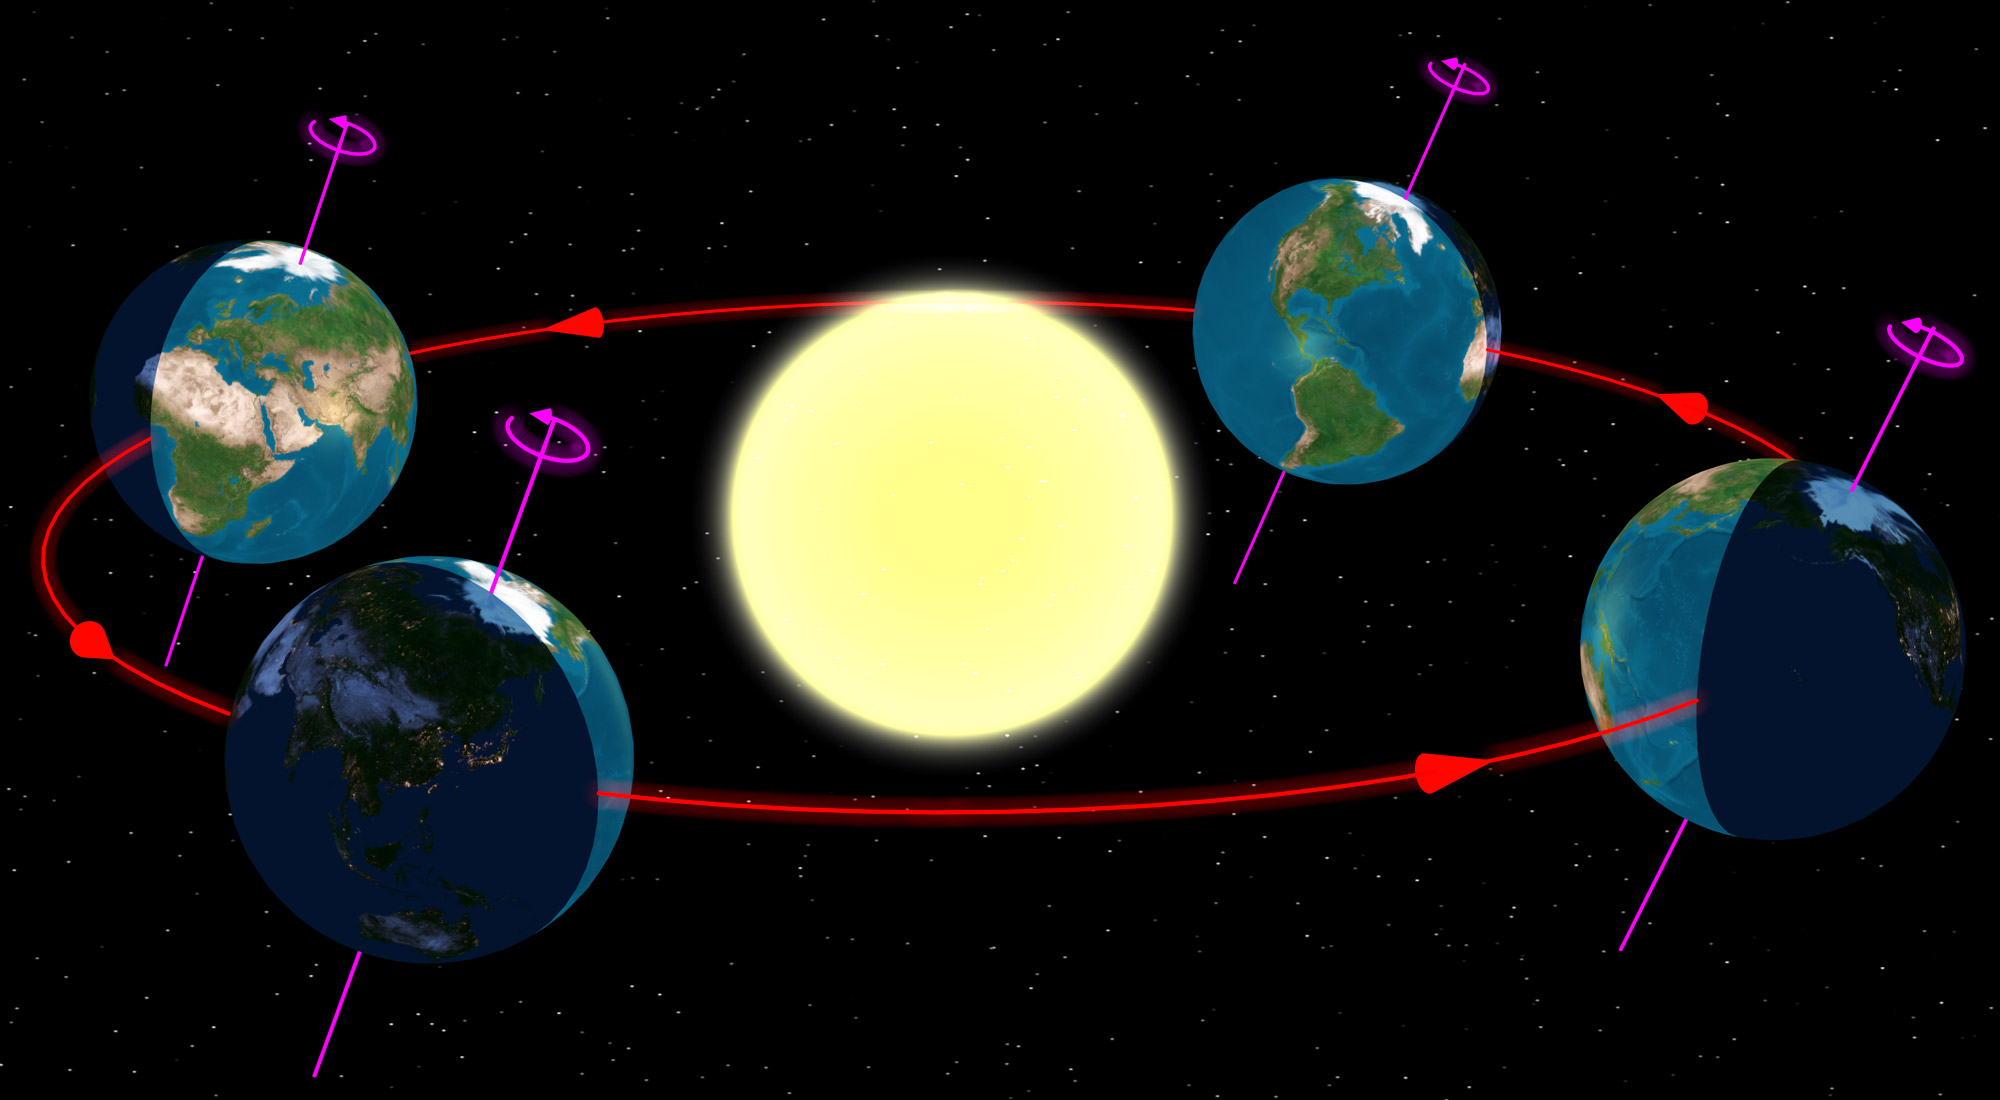
\includegraphics[width=\textwidth]{earth_orbit.jpg}
	\caption{ Earth orbiting the sun \protect\footnotemark}
\end{figure}
\footnotetext{\url{http://en.wikipedia.org/wiki/Summer_solstice}}

\begin{figure}[!h]
\center
	\label{fig:daylight_variation}
	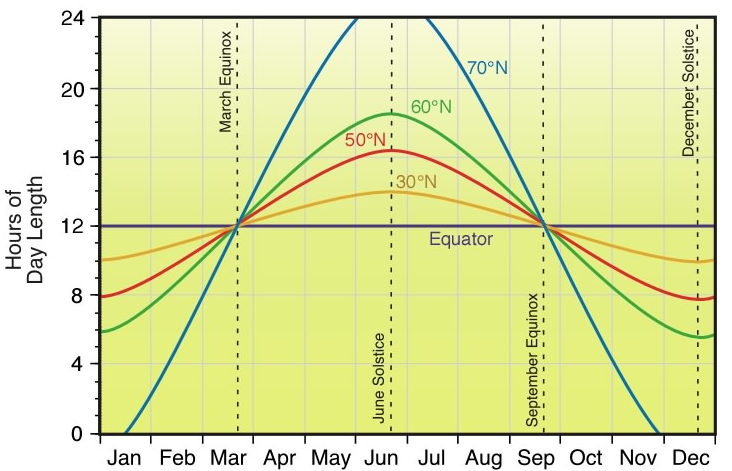
\includegraphics[width=\textwidth]{daylight_variation.png}
	\caption{ Variation in day length for different latitudes \protect\footnotemark}
\end{figure}
\footnotetext{\url{http://www.physicalgeography.net/fundamentals/6i.html}}

\begin{figure}[!h]
\center
	\label{fig:sun_rays}
	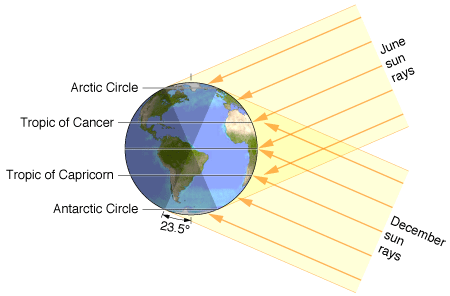
\includegraphics[width=\textwidth]{sun_rays_angles.png}
	\caption{ Sun rays angles \protect\footnotemark}
\end{figure}
\footnotetext{\url{http://physics.weber.edu/schroeder/ua/SunAndSeasons.html}}


\begin{table}[h]
  \centering
	  \label{tab:equinox_and_solstices}
	    \begin{tabular}{|p{3cm}|p{3cm}|p{3cm}|p{3cm}|p{3cm}|}
  	    \hline	
  	    \textbf{Name} & \textbf{Incidence angle at equator} & \textbf{Significance at equator} & \textbf{Significance for northern hemisphere} & \textbf{Significance for southern hemisphere} \\
		\hline
		\textbf{March equinox} & 0\textdegree & Sun vertical in the sky & - & - \\
		\hline
		\textbf{June solstice} & 23.5\textdegree & - &  longest day & shortest day \\
		\hline
		\textbf{September equinox} & 0\textdegree &  Sun vertical in the sky & - & - \\
		\hline
		\textbf{December solstice} & -23.5\textdegree & - & shortest day & longest day \\
		\hline
		\end{tabular}
		\caption{Key points during earth's orbit around the sun}
\end{table}

Rather than emulating earth's rotation around the sun, the system changes the reference frame and models the sun rotating around the earth. This simplifies the process as it permits the earth's position to remain static all year round. The sun's rotation axis is the earth's center axis (passing through both poles). A full rotation of the sun around this axis will represent 24 hours.\\
To replicate the variation of the sun's incidence angles, the earth's rotation axis varies between -23.5\textdegree at the December solstice (set to the 15$^{th}$ of December) to 23.5\textdegree at the June solstice (set to the 15$^{th}$ of June)
